\subsection{Smartphone}

\par 
El teléfono inteligente (smartphone en inglés) es un tipo de ordenador de bolsillo que combina los elementos de una tablet con los de un teléfono celular. Sobre una plataforma informática móvil, con mayor capacidad de almacenar datos y realizar actividades, semejante a la de una minicomputadora, y con una mayor conectividad que un teléfono móvil convencional. El término inteligente, que se utiliza con fines comerciales, hace referencia a la capacidad de usarse como un computador de bolsillo, y llega incluso a reemplazar a una computadora personal en algunos casos\cite{smartphone}.
	
\par \noindent
Generalmente, los teléfonos con pantallas táctiles son los llamados teléfonos inteligentes, pero el soporte completo al correo electrónico parece ser una característica indispensable encontrada en todos los modelos existentes y anunciados desde 2007\cite{smartphone}.
		
\par \noindent
Entre otros rasgos comunes está la función multitarea, el acceso a Internet vía Wifi o redes 2G, 3G o 4G, función multimedia (cámara y reproductor de videos/mp3), a los programas de agenda, administración de contactos, acelerómetros, GPS y algunos programas de navegación, así como ocasionalmente la habilidad de y leer documentos de negocios en variedad de formatos como PDF y Microsoft Office\cite{smartphone}.

\par \noindent
Los sistemas operativos móviles más frecuentes utilizados por los teléfonos inteligentes son Android (de Google), iOS (de Apple) y Windows 10 (de Microsoft)\cite{smartphone}.

\begin{figure}[H]
	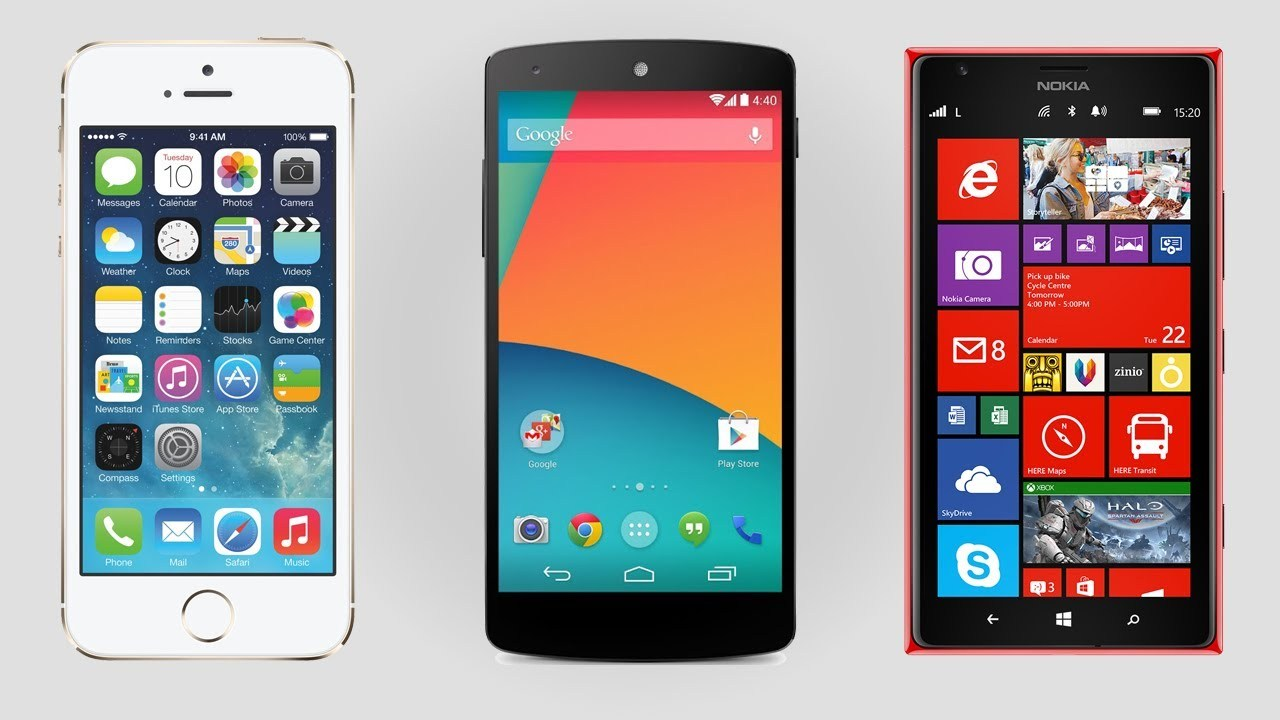
\includegraphics[width=\textwidth]{smartphone1.jpg}
	\caption{Smartphones con los Sistemas Operativos Móviles Mas Populares}
\end{figure}

\par \noindent
En nuestro trabajo utilizaremos exclusivamente para desarrollar el sistema operativo movil Android, debido a su popularidad en el mercado y su vasta documentación para desarrollar aplicaciones.